\subsection{``Price'' of spillover: sectoral and insdustry variation in potential for spillover}

As implied in the theory section, when the ``price'' of spillover is high (i.e. it is difficult to obtain spillover due to the country's absorptive capacity or sector-specific characteristics), the government official would choose a bundle that has more private benefit than spillover (\Cref{fig:price_of_spillover}). 

\begin{figure}[!ht]
	\centering
    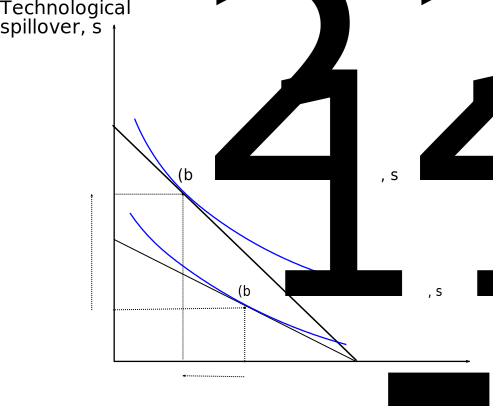
\includegraphics[width=0.75\textwidth, height=0.75\textheight,keepaspectratio]{../figure/price_of_spillover}
    \caption{As the ``price'' of spillover decreases, the official can get a larger amount of spillover given the same budget (i.e. the y-intercept of the budget constraint shifts up) Comparing the bundle $(s_1, b_1)$ and $(s_2, b_2)$, we see that the new bundle has more spillover and less bribe.}
    \label{fig:price_of_spillover}
\end{figure}

Here I focus on industry-specific characteristics that either facilitate or hinder spillover.\footnote{Absorptive capacity, or the ability of private firms to learn from their interaction with foreign firms, is also a very important factor in determining spillover. However, given the time-varying nature of absorptive capacity, not to mention the fact that official and firms can strategically invest to improve absorptive capacity, it is much harder to have a research design studying absorptive capacity that can claim exogeneity.} Due to the divisibility of its production process, manufacturing firms tend to engage more local suppliers and generate more spillover effect than primary and tertiary sectors. In addition, within each sector there is a wide variation across industries to be exploited as well. For example, in manufacturing, food processing can have a high amount of spillover due to the sourcing of raw materials and packaging, whereas in textile and automotive industries (which require high level of technological sophistication), it is harder for foreign firms to work with local suppliers. Similarly, in tertiary sectors, finance, trading, tourisms and utilities are is generally not divisible into discrete stages to subcontract. Yet service industries such as retailing and construction have more opportunities for input suppliers \citep[138]{UNCTAD2001}.

This leads us to the following hypothesis:

\begin{quote}
Hypothesis: Government official will pursue less bribe from firms in industries where it is easier to generate spillover
\end{quote}

While such variation across industries is clear conceptually, measurement is thorny given the many factors that can affect the potential for spillover. In addition, there is an endogeneity problem as the potential for spillover may itself be affected by the level of corruption in that industry. For example, an industry plagued by collusive relationship between the official and foreign firms does not offer an enabling environment that allows private firms to develop their absorptive capacity. The endogeneity problem is compounded if the official strategically decides whether to invest and improve absorptive capacity, in which case it is not even clear which direction is our estimate biased.

To address both of these measurement and endogeneity issues, I will use the variation in technological spillover across industries in the United States as the instrumental variable.\footnote{The United States is considered due to its high quality economic data. Alternatively, for each country, I can use a comparable country in the same region or the same developmental stage to formulate the instrument} The assumption is that the level of technological spillover in a US industry only correlates with the level of bribe in another country's industry through the latent factor that is the industry-specific potential for spillover.

\subsection{``Price'' of private benefit, i.e. cost of bribing for foreign firms}

As implied from the theory, when the ``price'' of private benefit is high (i.e. it is costly for the firm to offer the official private benefit), the official would choose a bundle that has less private benefit.

This theoretical claim generates many substantive predictions that we can test, each involving a factor that affects the cost of bribing for firms. For example, foreign firms that come from a corrupt home country may have more experience with bribing and thus would incur less information cost if they bribe.

Here I focus on the Phase 3 (Enforcement) of the OECD Anti-Bribery Convention (ABC) as an exogenous increase in the cost of bribing for foreign firms in Vietnam. In December 1997, all members of OECD and an additional five non-members, accounting for nearly 61\% of world trade, signed the ABC. The ABC criminalizes the bribery of foreign public officials and upholds its principles with a peer-monitoring system, in which member countries visit and review one another's legislation and implementation. According to legal experts, these reports are often quite harsh and effective in shaming countries into improving their practices \citep{Tyler2011}.

Important for my research design, in December 2009 the OECD's Working Group on Bribery (WGB) annouced that following Phase 1 and 2 (Evaluation and Assessment) there would be a Phase 3 (Enforcement). The goal of Phase 3 is to continually monitor countries' anti-bribery practices and to exhort inactive enforcers. Noticeably, Phase 3 also removed a previous exception that allowed firms to make ``small facilitation payment'' \citep{Strauss2013}. Researchers have argued that following the announcement of Phase 3, member countries ramped up enforcement to avoid a negative review, and causing their firms to reduce bribery abroad \citep{Malesky2015b}. 

Given that FDI to Vietnam only accounts for a small fraction of OECD countries' total foreign investment, it is plausible that Vietnam is not a major factor driving the initiation of Phase 3. Therefore, the announcement of Phase 3 serves as an exogenous shock to the cost of bribery for firms from ABC member countries. With OECD firms being reluctant to offer bribes, we expect corrupt officials to become uninterested in OECD firms. Post 2009, OECD firms would be attractive only to non-corrupt officials for their developmental impact, and we should observe them having more spillover effect.

With 2009 as an exogenous shock we have a difference-in-difference design. First, we estimate the difference in spillover between OECD and non-OECD firms, pre-2009. We then find the same difference in spillover post-2009. Subtracting these two differences, we can estimate the effect of corruption on the level of spillover.\footnote{An alternative design looks at the difference between OECD and non-OECD firms that \textit{enter} Vietnam pre- and post-2009. This design will have fewer firms in the sample but could be more appropriate if we think that the spillover-bribe bundle is negotiated at the time firms enter Vietnam and is hard to change later, even with the ABC coming into effect. If so, the change in level of spillover and bribe is caused by the change in the official's selection of firms instead of the adjustment in behaviors of existing firms after 2009.}

I sum, I have the following hypothesis:

\begin{quote}
Hypothesis: The Phase 3 (Enforcement) of OECD's Anti-Bribery Convention causes firms from member countries to have more spillover.
\end{quote}


\subsection{Time horizon of officials}

As implied by the theory above, an official with a longer time horizon would choose a bundle with more spillover, whereas an official with a short time horizon would choose a bundle with more private benefit.

To get a handle on the time horizon of the official, we need to know the options provided to the official within the country's political economic system. Such is a difficult question to study with a cross-national design due to endogeneity issues, stemming from unobservable and unmeasurable differences across political systems. Therefore, at this step, I focus on the case of Vietnam, whose large number of provincial units (63) and their variation in FDI flow serve as an excellent testing ground. Again, here I focus on bribe and informal fees as the main form of private benefit for officials. Such constraint is not problematic for the case of Vietnam, where the authoritarian system means that officials are not offered campaign contribution and where revolving door jobs are non-existent.

\subsubsection{The effect of time horizon on the choice of Vietnamese provincial officials} 

The relative weight assigned to spillover versus bribe by the Vietnamese provincial officials is determined by the principal-agent relationship between Vietnam's central and the provincial governments. On the one hand, the central government (i.e. the principal) cares more about the spillover effect of FDI and uses promotion to reward local officials that attract high-spillover FDI. On the other hand, local officials (i.e. the agent) have more opportunities to engage in corruption with foreign firms, and should they decide that the private benefit of corruption is greater than that of promotion, they will prioritize foreign firms that bring bribes over those that have high spillover effects.

The reason behind such difference in the preference of central and local governments is the fact that FDI projects are approved and managed at the provincial level. While the central law may be uniform in the book, its implementation varies widely across sub-national units in Vietnam \citep{Meyer2005}.\footnote{Vietnam's sub-national variation in implementation generalizes well to other cases, such as China \citep{Thun2006}} Therefore, provincial governments hold valuable services for sale to foreign firms. In contrast, the central government is more removed from direct contact with FDI firms and thus less likely to benefit from corruption than provincial leaders. 

In addition, the central government is much more concerned with overall economic growth, which is central to the longevity of the regime \citep{Malesky2008}. It wants to attract high-spillover FDI and uses promotion to reward local officials that accomplish this goal. On the other hand, each provincial leader is incentivized to free-ride on the developmental effort of other provinces and of the central to keep the entire regime stable. Therefore, local officials value the spillover effect of FDI only insofar as the opportunities for promotion that it brings.

Fortunately for the central government, the principal-agent problem in this context is partially solved because monitoring is not too difficult. Indeed, the central government can observe the economic performance of the provinces and use personnel management to punish and reward provincial officials \citep{Sheng2007, Li2005}.\footnote{\citet{Shih2012} recently argue that economic performance does not matter to cadre promotion. However, they investigate all members of the Chinese Central Committee, including the central party apparatus, the army, and the central economic bureaucracy. These actors are not the important decision-makers in our theory.} Therefore, the principal-agent problem is only severe when provincial officials are not interested in further promotion to the central government, i.e. when the local official's time horizon is short. This suggests that there will be a variation in the level of FDI's spillover effect across provinces according to provincial officials' interest in promotion. In the research design, I use fuzzy regression discontinuity (RD) exploiting the mandated retirement age of Vietnamese officials, arguing that those that are in their last term have shorter time horizon and less interest in promotion.\footnote{The design is \textit{fuzzy} RD because the shortening of time horizon does not happen so abruptly as after a specific date. Instead, it happens in a time window after the official enters their last term before retirement.}

By looking at this variation in the career interest of provincial officials, my theory contributes a fresh angle to the current literature on the relationship between decentralization and corruption. So far, scholars have only postulated a one-way relationship: either decentralization increases bribery \citep{Fan2009} or reduces it \citep{Guerra2009}. In my model, how decentralization affects corruption is conditional on the local officials' interest in the promotions offered by the central as carrots.


Three key assumptions in the theory above deserve further examination:
\begin{enumerate}
\item Why wouldn't Vietnam's central government worry that technological spillover would lead to a developed private sector, and consequently to social change that ultimately undermines its rule?

First, there is a large scholarship showing that authoritarian regimes are very adept at using institutions to manage regime outsiders in general and business in particular \citep{Gandhi2006, Gandhi2008, Wright2008, Le2015}. Second, if the legitimacy of the regime rests heavily on delivering economic growth, then the short-term risk of an economic downturn creating instability features much more prominently than the long-term concern with social changes. Third, it is possible to foster economic growth while restricting political freedom (e.g. Singapore). Indeed, growth can make a regime, both democratic and authoritarian, more stable, and creates room for political control \citep{Przeworski1997}.

\item Why don't provincial leaders seek rent from the domestic sector? 

First, Vietnam's private sector was very small when FDI was first allowed into Vietnam. The size and the profitability of the average domestic firm is still smaller than those of foreign firms today. Therefore, there are both fewer rents and more coordination problems if provincial officials want to seek rents from domestic firms. Second, ironically, if officials want to grow the private sector for future rent-seeking, they must promote an enabling business environment that are free from rent-seeking. In contrast, engaging in corruption with large and existing FDI firms is much more convenient. Essentially, corrupt provincial officials have shifted the cost of building a thriving domestic sectors to the home countries of FDI firms and now extract rents from the high productivity and high profitability of these firms. 
\end{enumerate}

In sum, I propose a hypothesis about variation across Vietnam's provinces:

\begin{quote}
Hypothesis: In provinces whose leaders are in their last term before the mandated retirement age, there are more spillover and less bribe from the foreign firms.
\end{quote}
